% !TEX root=meca1321-synthesis.tex
\tikzsetnextfilename{Hagen}
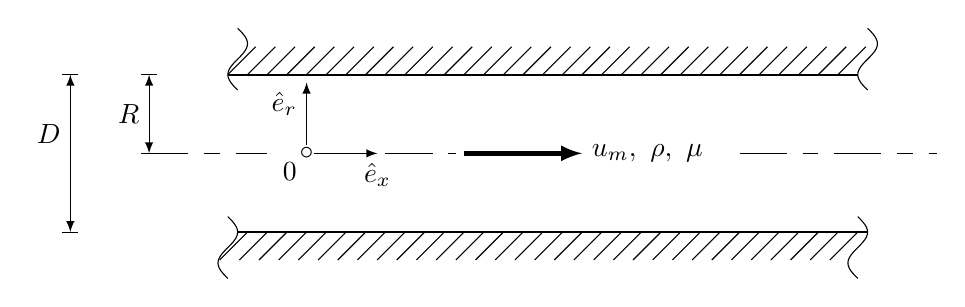
\begin{tikzpicture}
  % Tracé des parois
  \draw [thick] (-4,1) -- (4,1);
  \draw [domain=-pi:pi] plot ({sin(deg(\x))/8-3.875},{((\x+pi/2)/8+1});
  \draw [domain=-pi:pi] plot ({sin(deg(\x))/8+4.125},{((\x+pi/2)/8+1});
  \draw [thick] (-3.875,-1) -- (4.125,-1);
  \draw [domain=-pi:pi] plot ({sin(deg(\x))/8-4},{((\x-pi/2)/8-1});
  \draw [domain=-pi:pi] plot ({sin(deg(\x))/8+4},{((\x-pi/2)/8-1});
  \foreach \i in {0,...,31}
  {
    \pgfmathsetmacro{\x}{(- 4 + \i/4)};
    \draw (\x,1) -- ++(45:0.5);
    \draw (\x+1/4,-1) -- ++(-135:0.5);
  }
  %Repères et autres flèches
  \draw [dash pattern= on 0.6cm off 0.2cm on 0.2cm off 0.2cm] (-5.1,0) -- (-3.5,0);
  \draw [>=latex,<->] (-6,-1) -- (-6,1);
  \draw (-5.1,1) -- ++(0.2,0);
  \draw (-5,0.5) node [left] {$R$};
  \draw [>=latex,<->] (-5,0) -- (-5,1);
  \draw (-6.1,1) -- ++(0.2,0);
  \draw (-6.1,-1) -- ++(0.2,0);
  \draw (-6,0) node [above left] {$D$};
  \draw (-3,0) node {$\circ$};
  \draw (-3,0) node [below left] {$0$};
  \draw [>=latex,->] (-3,0.1) -- (-3,0.9);
  \draw [>=latex,->] (-2.9,0) -- (-2.1,0);
  \draw (-3.0,0.9) node [below left] {$\hat{\vb{e}}_r$};
  \draw (-2.1,0) node [below] {$\hat{\vb{e}}_x$};
  \draw [dash pattern= on 0.6cm off 0.2cm on 0.2cm off 0.2cm] (-2,0) -- (-1.1,0);
  \draw [ultra thick,>=latex,->] (-1,0) -- (0.5,0);
  \draw (0.5,0) node [right] {$u_m,~\rho,~\mu$};
  \draw [dash pattern= on 0.6cm off 0.2cm on 0.2cm off 0.2cm] (2.5,0) -- (5,0);
\end{tikzpicture}
